\chapter{Introducció}

El \textit{boom} de la \ac{IA} dels darrers anys és fruit de la convergència de diversos factors: la disponibilitat massiva de dades digitals, l'augment exponencial de la capacitat de còmput gràcies a les unitats de processament gràfic (GPU), i la inversió que any rere any augmenta  tant des del sector privat com des de l'àmbit públic. En poc més d'una dècada, els sistemes basats en aprenentatge automàtic han passat de ser objecte de recerca de laboratori a integrar-se de manera natural en el dia a dia: assistents de veu, sistemes de recomanació, diagnosi mèdica assistida, conducció autònoma o detecció de fraus financers, suposant això un impacte directe sobre el teixit econòmic i productiu \cite{Arco25}. L'abast d'aquesta transformació no té precedents en la història de la tecnologia, i planteja reptes que van molt més enllà de la millora del rendiment dels models.

Un d'aquests reptes és el que constitueix el nucli d'aquest treball: entendre \emph{per què} un model d'IA pren una determinada decisió. La qüestió no és trivial. Els models d'aprenentatge profund que ofereixen les millors prestacions com les xarxes neuronals amb milions o fins i tot milers de milions de paràmetres operen com a \emph{caixes negres}: reben una entrada, realitzen transformacions no lineals en espais de dimensions molt elevades, i produeixen una sortida. El mecanisme intern és, en la majoria dels casos, opac fins i tot per als seus creadors degut a l'alt nombre d'operacions que executen. L'\ac{XAI} sorgeix precisament com a resposta a aquesta opacitat: una disciplina que busca fer que certs aspectes d'un sistema intel·ligent puguin ser comprensibles per als éssers humans, independentment de que siguin desenvolupadors, dissenyadors, reguladors o usuaris en general.

La importància de l'explicabilitat s'il·lustra millor amb un exemple concret que amb definicions abstractes. Considerem el camp de la medicina, on la \ac{IA} té un potencial transformador enorme en un context on la saturació de les cues sanitàries és un problema real. Un model de classificació que identifiqui automàticament símptomes lleus com un refredat comú, per exemple, pot alleujar la pressió sobre els serveis d'urgències i augmentar l'eficiència del sistema sanitari. Si comet un error en aquest cas, les conseqüències solen ser manejables: el pacient rebrà atenció mèdica per una altra via. Ara bé, quan el sistema analitza una radiografia per detectar la presència d'un tumor maligne, la situació canvia radicalment. Un fals negatiu pot costar una vida i un fals positiu pot sotmetre un pacient a tractaments agressius innecessaris. En aquest context, no n'hi ha prou amb saber que el model encerta el 95\% de les vegades; cal entendre \emph{en quines regions de la imatge} es basa per arribar a la predicció. Sense aquesta informació, el metge no pot validar ni refutar el diagnòstic de la màquina, i la col·laboració entre un expert humà i el sistema d'IA queda fonamentada en la fe cega, no en el raonament informat.

L'exemple mèdic no és una excepció: la mateixa lògica s'aplica a la concessió de crèdits bancaris, on la normativa europea, concretament el Reglament General de Protecció de Dades (RGPD) i, més recentment, la legislació europea relativa a la IA recollida a \cite{EUAIAct24}, obliga a les institucions financeres a proporcionar explicacions comprensibles per a les decisions automatitzades que afecten les persones. O a la conducció autònoma, on un error de classificació pot tenir conseqüències fatals en fraccions de segon. O als sistemes de selecció de personal, on les decisions de categorització de candidats poden estar influïdes per biaixos negatius enlloc de característiques professionals reals. En tots aquests àmbits, l'explicabilitat no és un element opcional ni cosmètic: és un requisit d'enginyeria tant com un principi ètic que fomenta l'ús de models més robusts.

La comunitat científica ha respost a aquesta demanda amb una proliferació notable de mètodes. Alguns operen sobre el model sencer, buscant una comprensió global del seu comportament; d'altres s'orienten a explicar prediccions individuals, de manera local. Alguns s'apliquen sobre models ja entrenats com els anomenats mètodes \emph{post-hoc}: LIME, SHAP o Integrated Gradients; d'altres, anomenats mètodes \emph{ante-hoc} incorporen l'explicabilitat directament en el disseny del model, com els arbres de decisió. La diversitat d'aproximacions és un indicador de la maduresa del camp, però simultàneament genera un problema nou: com sabem quin mètode d'explicació és millor? Com avaluem la qualitat d'una explicació?

Un exemple il·lustratiu d'aquesta problemàtica prové d'un estudi clàssic en el camp de la \ac{XAI} \cite{Tulio16}. Un model de classificació d'imatges entrenat per distingir entre llops i huskies siberians assoleix una precisió molt elevada en el conjunt de test. Tanmateix, quan s'analitzen les explicacions del model mitjançant tècniques de visualització d'atribució, s'observa que el model no aprèn a reconèixer les característiques morfològiques dels animals com la forma del morro, el color del pelatge o les proporcions corporals, sinó el \emph{fons de la imatge}: les imatges de llops solen aparèixer en paisatges nevats, mentre que les de huskies apareixen en entorns boscosos o domèstics. El model ha après un \emph{shortcut}\cite{Longo2024}: una correlació espúria entre el fons i l'etiqueta que funciona bé sobre les dades d'entrenament però que fallaria estrepitosament en producció si se li presentés un husky en un paisatge nevat (Figura ~\ref{fig:husky}) i planteja una pregunta: el model aprèn realment el que és un llop?

\begin{figure}
\begin{center}
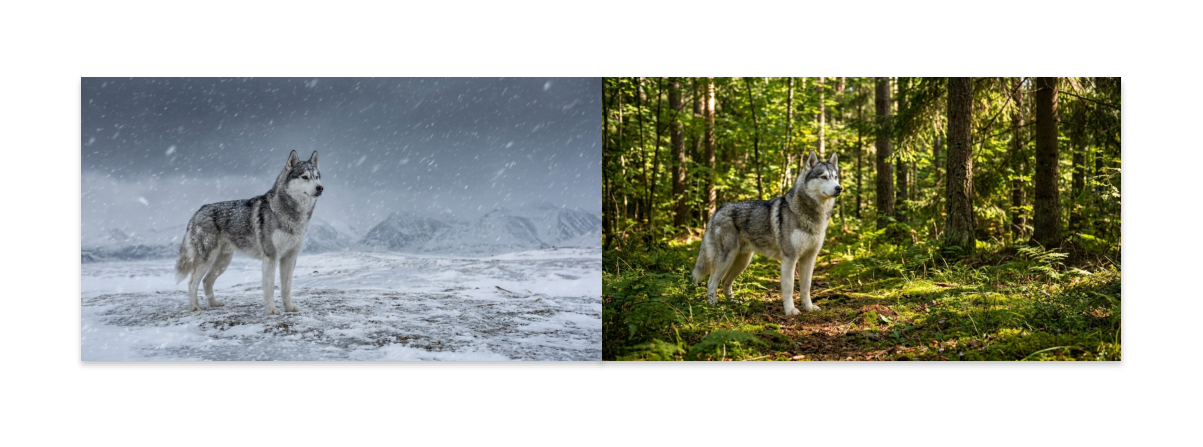
\includegraphics[width=0.9\textwidth]{./figures/introduccio/husky.pdf}
\caption{El mateix husky siberià en dos contextos diferents: paisatge nevat (esquerra) i bosc (dreta). Un model sense explicabilitat podria classificar la imatge de l'esquerra com a \textit{llop} basant-se en el fons, no en l'animal.}
\label{fig:husky}
\end{center}
\end{figure}

Sense eines d'explicabilitat, aquest comportament seria completament indetectable: el model retorna una etiqueta i una probabilitat, però no ofereix cap indici de quina informació de l'entrada ha determinat la seva decisió. Amb un mètode \ac{XAI} d'atribució de característiques, el mapa de calor resultant posa de manifest que el model ignora l'animal i focalitza l'atenció en la neu del fons. D'aquesta manera ens trobem davant d'una caixa negra que, per primer cop, es pot il·luminar.

\section{Motivació i objectius}
L'avaluació dels mètodes \ac{XAI} és precisament la pregunta on radica el problema obert que motiva aquest treball. \cite{Hesse2023} constata que un terç dels articles sobre \ac{XAI} manca d'una avaluació quantitativa sòlida, i que els protocols d'avaluació existents sovint presenten problemes de comparabilitat o introdueixen imatges fora de la distribució d'entrenament del model, cosa que pot distorsionar els resultats. \cite{Ariasduart2022} posa de manifest que una avaluació qualitativa sola basada en la percepció humana no pot garantir que les explicacions siguin fidels al comportament real del model. En altres paraules: una explicació pot semblar coherent i entenedora per a un humà i ser, a la vegada, completament infidel al mecanisme intern del sistema. 

L'elecció d'aquest tema com a \ac{TFG} respon a tres motivacions que es complementen. En primer lloc, un interès personal sostingut per la pregunta de fons que travessa tota la disciplina: \emph{per què un sistema complex actúa com actúa}? El camp de la \ac{XAI} tracta específicament aquesta qüestió i ho fa amb un objectiu, entre d'altres, que consider essencial en les noves tecnologies que es desenvolupen avui en dia: afavorir els avenços èticament auditables. En segon lloc, la voluntat de tancar els estudis universitaris amb un treball que vagi més enllà de la implementació tècnica i que plantegi una pregunta de recerca oberta, contribuint modestament a un debat actiu en la comunitat científica. Això implica fer una recerca exhaustiva de l'estat de l'art de la matèria i exigeix certa creativitat acadèmica a l'hora de pensar solucions. En tercer lloc, la utilitat directa que les metodologies i troballes explorades en aquest document poden tenir per al treball en curs de \textbf{referència a voltros}, els meus co-tutors, amb qui es comparteix el marc teòric i l'interès pel camp de la explicabilitat.

Aquest treball s'emmarca en aquesta problemàtica i té una naturalesa dual que convé fer explícita des del principi deguda a la meva especialització acadèmica. D'una banda, és un \emph{projecte d'enginyeria}: s'ha definit un plà per assolir uns objectius concrets guiat per unes mètriques que s'aclareixen mes endavant. Per assolir aquests objectius s'ha dissenyat i implementa un \emph{pipeline} que ha anat millorant-se de forma iterativa en funció de si els resultats que s'han anat obtenint esteien alineats amb l'objectiu final del projecte i eren útils. Aquest \emph{pipeline} automatitzat consisteix en generar un dataset d'imatges fotorealistes amb intervencions controlades, integrant segmentació semàntica amb SAM~2, múltiples backends d'inpainting (LaMa, Replicate i NanoBanana, basat en Imagen~4 de Google), i el càlcul sistemàtic de mètriques de qualitat d'imatge. Tot això per a obtenir un conjunt de dades sintètic que ens permeti fer un estudi aplicant algunes tècniques d'explicabilitat. 

D'altra banda, és un \emph{treball de recerca acadèmica} que també es planteja si les mètriques convencionals de qualitat, similitud estructural, divergència de píxels i coherència de píxels exteriors, constitueixen predictors fiables de la utilitat dels mètodes \ac{XAI} quan s'apliquen sobre les imatges manipulades. La hipòtesi de partida és que millors mètriques no impliquen necessàriament millors inputs per a l'avaluació de l'explicabilitat, a la vegada que s'explora la dissociació entre qualitat perceptual i mètriques quantitatives que s'observarà experimentalment.

La inspiració metodològica prové de \cite{Hesse2023}, un dataset sintètic de classificacions d'ocells artificials que permet avaluar mètodes \ac{XAI} mitjançant intervencions semàntiques controlades com l'eliminació d'una ala o el bec d'un ocell i comparar les explicacions del model amb importàncies de parts calculades com a \textit{ground truth}. El present treball adopta el mateix esperit metodològic, però opera sobre imatges fotorealistes del dataset COCO. Això introdueix una complexitat afegida significativa: les imatges reals presenten variabilitat de textura, il·luminació i context que els entorns sintètics eludeixen per construcció. El repte és, però, precisament aquí: validar si les eines d'avaluació de \ac{XAI} desenvolupades en entorns controlats són traslladables a condicions més properes al desplegament real dels models. 

\section{Estructura de la memòria}
Al llarg d'aquest \ac{TFG} s'hi troba condensat tot el reflex de la de recerca i desenvolupament tècnic necessaris per a respondre les qüestions anteriorment formulades. En el pròxim capítol \ref{analisi} es presenta l'anàlisi del problema i es justifica la manera d'enfocar la feina, incidint en les metodologies que s'han usat per assolir aquest projecte. D'aquesta forma, s'estableix una guia al lector que ajuda a entendre i comprendre millor el procés de recerca i desenvolupament que s'ha seguit.

Posteriorment, ens endinsarem i aclarirem els aspectes teòrics, des dels més bàsics fins als més complexos al capítol \ref{teoria}. Aquest apartat serà la referència acadèmica a la que m'estaré referint al llarg de la fase de desenvolupament i estudi dels resultats per a fer una aportació actualitzada a l'estat de l'art del camp. Conté els fonaments dels models de classificació per visió, tècniques d'inpainting generatiu, descripció dels mètodes \ac{XAI} emprats, en particular els Gradients Integrats, i la definició de les mètriques de qualitat utilitzades.

Un cop situats els objectius acadèmics i el panorama actual en el món de la investigació, es presenta el capítol d'\ref{experimentacio}. Aquest n'és el més extens degut a que descriu el procés experimental complet: disseny del pipeline, selecció d'imatges, generació del \emph{dataset}, càlcul de mètriques i aplicació dels mètodes \ac{XAI}, incloent-hi la discussió de la dissociació observada entre qualitat perceptual i mètriques quantitatives.

Finalment, el darrer capítol recull les \ref{conclusions} del treball, les seves limitacions i les línies de recerca futures que obre.
